\documentclass[conference]{IEEEtran}
\IEEEoverridecommandlockouts
\usepackage[boldmath]{numprint}
\usepackage[inkscapeformat=png]{svg}
\usepackage{cite}
\usepackage{amsmath,amssymb,amsfonts}
\usepackage{algorithmic}
\usepackage{graphicx}
\usepackage{textcomp}
\usepackage{xcolor}
\usepackage{multirow}
\usepackage{booktabs}
\usepackage{hyperref}

\def\BibTeX{{\rm B\kern-.05em{\sc i\kern-.025em b}\kern-.08em
    T\kern-.1667em\lower.7ex\hbox{E}\kern-.125emX}}
\begin{document}

\title{Data Driven Derivative-based Regularization for Regression}

\author{
\IEEEauthorblockN{1\textsuperscript{st} Anonymous}
\IEEEauthorblockA{\textit{Anonymous} 
}

\and 

\IEEEauthorblockN{2\textsuperscript{nd} Anonymous}
\IEEEauthorblockA{\textit{Anonymous} \\
}
\and 

\IEEEauthorblockN{3\textsuperscript{rd} Anonymous}
\IEEEauthorblockA{\textit{Anonymous} \\
}
\and 

\IEEEauthorblockN{4\textsuperscript{th} Anonymous}
\IEEEauthorblockA{\textit{Anonymous} \\
}

\and 

\IEEEauthorblockN{5\textsuperscript{th} Anonymous}
\IEEEauthorblockA{\textit{Anonymous} \\
}


}

\maketitle



\begin{IEEEkeywords}
Machine Learning, Neural Networks, Regularization, Regression, DLoss, Data Derivative
\end{IEEEkeywords}


\begin{abstract}
In this work, we introduce a novel approach to regularization in multivariable regression problems. 
Our regularizer, called \emph{DLoss}, penalizes differences between the model's derivatives and derivatives of the data generating function as estimated from the training data. 
We call these estimated derivatives \emph{data derivatives}. 
The goal of our method is to align the model to the data, not only in terms of target values but also in terms of the derivatives involved. 
To estimate data derivatives, we select (from the training data) 2-tuples of input-value pairs, using either nearest neighbor or random selection. 
We evaluate the effectiveness of \emph{DLoss} on synthetic and real datasets with different weights, to the standard mean squared error loss. 
The experimental results show that with \emph{DLoss} (using nearest neighbor selection) we obtain, on average, the best rank with respect to MSE on validation data sets, compared to no regularization, $L_2$ regularization, and Dropout. 
Our implementation code is available on Github.
\end{abstract}

\nopagebreak
\section{Introduction}
\label{introduction}

Regularization is used by many different methods in statistics, inverse problems, and machine learning, to prevent overfitting and numeric instability when a model is fitted to data \cite{Kukacka2017regsurvey}.
Traditional regularization methods use an additional term in the loss function used during model training, where this additional term is based on the model parameters. 
Most frequently used are the $L_1$ \cite{tibshirani1996L1} and $L_2$~\cite{TikhonovL2} norms of model parameters (i.e., norms of the coefficients of a linear model or the weights of a neural network). 
Another widely used regularization method (but only for neural networks) is \emph{DropOut}, where there is no additional loss term while neurons are randomly switched off during training~\cite{hinton2012L2,srivastava2014dropout}.

The distinguishing feature of all these regularizers is that they do not explicitly use characteristics of the unknown target function, where these characteristics may be inferred from training data. 
In this paper, we propose a novel regularization approach for regression, called \emph{DLoss}, that (a) is derived from training data, and (b) is applicable to any type of model where one can specify a loss function.
\emph{DLoss} is formulated as a term in the loss function that penalizes the difference between a model derivative and a derivative estimated from data points. 

Our contributions are:
\begin{enumerate}
 \item We propose a new regularization method for regression models, \emph{DLoss};
 \item We propose two variants of \emph{DLoss} using nearest neighbor or random selection of data points;
 \item We provide a publicly available implementation in PyTorch;
 \item We evaluate our approach on different datasets and compare it to training using MSE without regularization, with $L_2$ regularization, and with Dropout.
\end{enumerate}
The results show that \emph{DLoss} leads on average to better generalization results at a moderate increase of the computational cost. 

The paper is structured as follows.
In \autoref{sec:related}, we discuss related work on regularization and differential equations. 
In \autoref{sec:method}, we introduce our method. 
In \autoref{sec:experiments}, we describe the setup of our experiments. 
In \autoref{sec:results}, we present and discuss the experimental results, and in \autoref{sec:conclusion} we draw conclusions and discuss possible future work.

%%%%%%%%%%%%%%%%%%%%%%%%%%%%%%%%%%%%%

\section{Related Work}\label{sec:related}

Our method uses information derived from the data and is not specific to any model type as opposed to common regularization approaches.
Since we are using the derivatives in our approach we also overview the related work on Neural Differential Equations.

\subsection{Regularization}
Regularization aims to improve generalization \cite{Kukacka2017regsurvey}.
The most common regularization methods, $L_1$ and $L_2$ loss on the parameters, are also called \emph{weight decay} when applied to neural networks.
In generalized linear models and neural networks, lower weights lead to smaller gradients of the model function with respect to the inputs. 
Intuitively speaking, preferring smaller gradients means that flat and smooth functions are preferred. 
This preference is independent of the training data.

\emph{DropOut} is another popular regularization technique and is specific to neural networks. 
It works by switching off neurons at random during training~\cite{srivastava2014dropout,baldi2013understanding}. 

\subsection{Neural Networks, Derivatives and Differential Equations} 

Our model adds differential terms to the loss function. 
While we believe that this our approach is novel, there are various types of models in the literature that integrate differential equations with neural networks. 

\textbf{Approximating derivatives of known functions} by neural networks 
was already studied by \cite{hornik-et-al-1990-universal} who showed that neural networks can approximate functions and their derivatives. 
This approach assumes that the derivatives of the approximated function are known, and a modification of the network architecture is required in order to achieve the approximation. 
A more recent approach to approximating a known function with neural networks has been presented in \cite{Avrutskiy2017}, which operates similar to our approach and does not require a change to network architectures. 
It extended to higher-order derivatives in 
\cite{Avrutskiy2021}. 

\textbf{Integrating prior knowledge} by using derivatives was, to the best of our knowledge, first introduced in
\cite{LeCun91} as \emph{tangent prop}. 
Tangent prop integrates prior knowledge about invariances into the network: the network is trained using desired directional derivatives of a target function with respect to the changes in the inputs. 
This is used in the context of image classification to encourage small derivatives in directions where changes of the inputs should not affect the output. 
For example, for handwritten digits, rotations by a small amount should not affect the class output. 
Tangent prop results in a fitted neural network that approximates the desired differential behavior. 

This approach has, in recent years, been re-kindled in the more general framework of physics-informed neural networks (PINNs) \cite{raissi2019physics,cuomo2022scientific}, which injects knowledge from physics into neural networks, in the form of differential equations. 

\textbf{Numeric solutions to differential equations} by neural networks have been used since the 1990s. 
Early work by \cite{lee1990neural} already introduced this approach, more recent examples are \cite{parisi2003solving} and \cite{malek2006numerical}, and an overview can be found in \cite{beck2023overview}.

\textbf{Neural differential equations} (NDE) are a more recent approach to unify neural networks with differential equations for an overview, see \cite{Kidger22}.
A neural ordinary differential equation (NODE) \cite{NEURIPS2018_Chen} estimates a continuous-time function that defines an ordinary differential equation (ODE), where this ODE approximates the discrete-time behavior of a recursive process (such as an RNN). In essence, the recursive mapping of inputs to outputs is approximated by motion along the solution to the ODE~--- i.e., motion along a vector field.
Neural stochastic differential equations (NSDE) \cite{tzen2019neural} define diffusion processes, rather than vector fields. 
They are also used to learn continuous-time models, but of \textit{stochastic} recurrent processes. 
In contrast, for our work, we assume the target function is continuously differentiable and its differential characteristics can be estimated from data. 


%%%%%%%%%%%%%%%%%%%%%%%%%%%%%%%%%%%%%

\section{Derivative-based Regularization Method}\label{sec:method}

In this study, we introduce a regularization term that aims to align model derivatives with estimated derivatives of the target function.
This approach is data driven, and does not impose a prior on the model parameters. 
Notwithstanding the increasing use of differential equations in combination with neural networks, this form of regularization is, to the best of our knowledge, proposed here for the first time.

\subsection{Intuition}
Our regularizer aligns model derivatives with estimated derivatives of the unknown, true, target function that generated the data.
By considering derivatives of the target (estimated from training data), in addition to the target values, our approach seems intuitively more promising than other regularization approaches that rely solely on target values, and more generally applicable than approaches that rely on prior knowledge of the target's differential characteristics.

For our regularizer, the following information is needed.
Firstly, it needs derivatives of the model with respect to the input.
These derivatives may be calculated analytically, or can be approximated by a finite difference approach given the model.
Secondly, it needs estimates of target function derivatives with respect to the input, which we estimate with a simple finite-difference approach. 
We want to minimize the difference between the model derivative and the estimated target derivative; i.e., we want to minimize the value of a \emph{DLoss} function, which we will define.

\subsection{Regression}
\label{subsec_regressiontasks}

We focus on \emph{regression problems}, that is, the approximation of an unknown, continuous, real-valued target function with $k$ arguments, $g(\cdot):{\mathbb R}^{k}\to{\mathbb R}$, by a model, $f(\cdot,\boldsymbol{\beta}):{\mathbb R}^{k}\to{\mathbb R}$, parameterized by a vector $\boldsymbol{\beta}\in{\mathbb R}^m$. 
Using training data consisting of input-output pair $(\mathbf{x}_i,y_i)$ (for $i=1,\ldots,n$, where $n$ is the number of training data points), regression modeling aims to optimize the parameter vector $\boldsymbol{\beta}$ of this function $f$, so that for general input-output pair $(\mathbf{x},y)$, 
\begin{equation}
 f(\mathbf{x},\boldsymbol{\beta}) = \hat{y}
\end{equation}
approximates the unknown function $g(\mathbf{x})=y$ sufficiently well. 
The variable $\mathbf{x}\in\mathbb{R}^k$ is called an 

\textit{independent variable vector} in statistics, and called \textit{feature} or \textit{input vectors} in machine learning. The corresponding $y \in \mathbb{R}$, that satisfies $g(\mathbf{x})=y$, is the \textit{dependent variable}, \textit{response variable} or \textit{target}.
In this paper, we refer to an input vector $\mathbf{x}$ as a point, $(\mathbf{x},y)$ as a pair, and two pairs $((\mathbf{x}_i,y_i),(\mathbf{x}_j,y_j))$ as a tuple.


For a given parameter vector $\boldsymbol{\beta}$, the model makes a prediction, $\hat{y}_i = f(\mathbf{x}_i,\boldsymbol{\beta})$, for the $i$th training input $\mathbf{x}_i$.
In general, it is expected that $\hat{y}_i$ will differ from the target value $y_i$. The task is to determine a preferred $\boldsymbol{\beta}$, via training using $(\mathbf{x}_i,y_i)$ pairs, that minimizes a suitable loss function; i.e., minimizes a suitable measure of the error between the predicted values $\hat{y}_i$ and target values $y_i$. 
One has ``fitted the model to the data'' when a preferred $\boldsymbol \beta$ has been determined.

The standard loss function to optimize is the \emph{mean squared error} (MSE) (i.e., the mean of the squared residuals):

\begin{equation}
 MSE = \frac{1}{n}\sum_{i=1}^n (y_i - f(\mathbf{x}_i,\boldsymbol{\beta}))^2\,.
\end{equation}

In standard multivariable linear modeling, we assume $y = g(\mathbf{x}) + \epsilon $, where $\epsilon$ is a normally distributed random variable representing noise, in which case the solution that optimizes the MSE (the least squares solution) also maximizes the likelihood of the data see, e.g., \cite{hastie01statisticallearning}.
We optimize $\boldsymbol{\beta}$ using only the training data~--- a separate \emph{validation dataset} is used to assess how well the fitted model performs on data (specifically, model inputs) it was not trained on. 
It is common to find that the value of $\boldsymbol{\beta}$ that gives the best model performance on the training set does not give good model performance on the validation set, which is called overfitting. 

\subsection{Regularization}
Traditional regularization discourages overfitting as follows: during model training, an additional term to the loss function helps find a parameter vector, $\boldsymbol{\beta}$, that ensures $f(\cdot,\boldsymbol{\beta})$ approximates the unknown target function well on unseen data from the same data distribution see, e.g., \cite{Kukacka2017regsurvey}.
The most common additional terms are the $L_1$ norm and the squared $L_2$ norm of the parameter vector (denoted $\|\boldsymbol{\beta}\|_1\mbox{ and } \|\boldsymbol{\beta}\|_2^2$). These terms are typically applied with a coefficient $\theta \in \mathbb{R}$, that regulates how much large weights (i.e., large model parameters) are penalized, so that the total loss $L$ is
\begin{equation}
 L = \theta \|\boldsymbol{\beta}\|_i^i + MSE\,,\quad\mbox{for }i \in \{1,2\}.
\end{equation}
Both $L_1$ and $L_2$ norms encourage the weights to be as small as possible.
The $L_1$ norm, $\|\boldsymbol{\beta}\|_1 = \sum_{j=1}^m |\boldsymbol{\beta}_j|$, corresponds to a Laplacian prior with 0 mean \cite{williams1995bayesian,plaut86,tibshirani1996L1}. The $L_2$ norm, $\|\boldsymbol{\beta}\|_2 = \sqrt{ \sum_{j=1}^m \boldsymbol{\beta}_j^2}$, corresponds to a Gaussian prior with 0 mean and standard deviation $\theta^{-1}$ \cite{rennie2003l2,Bishop95}.
 

%%%%%%%%%%%%%%%%%%%%%%%%%%%%%%%%%%%%%

\begin{figure}[t]
 \centering
 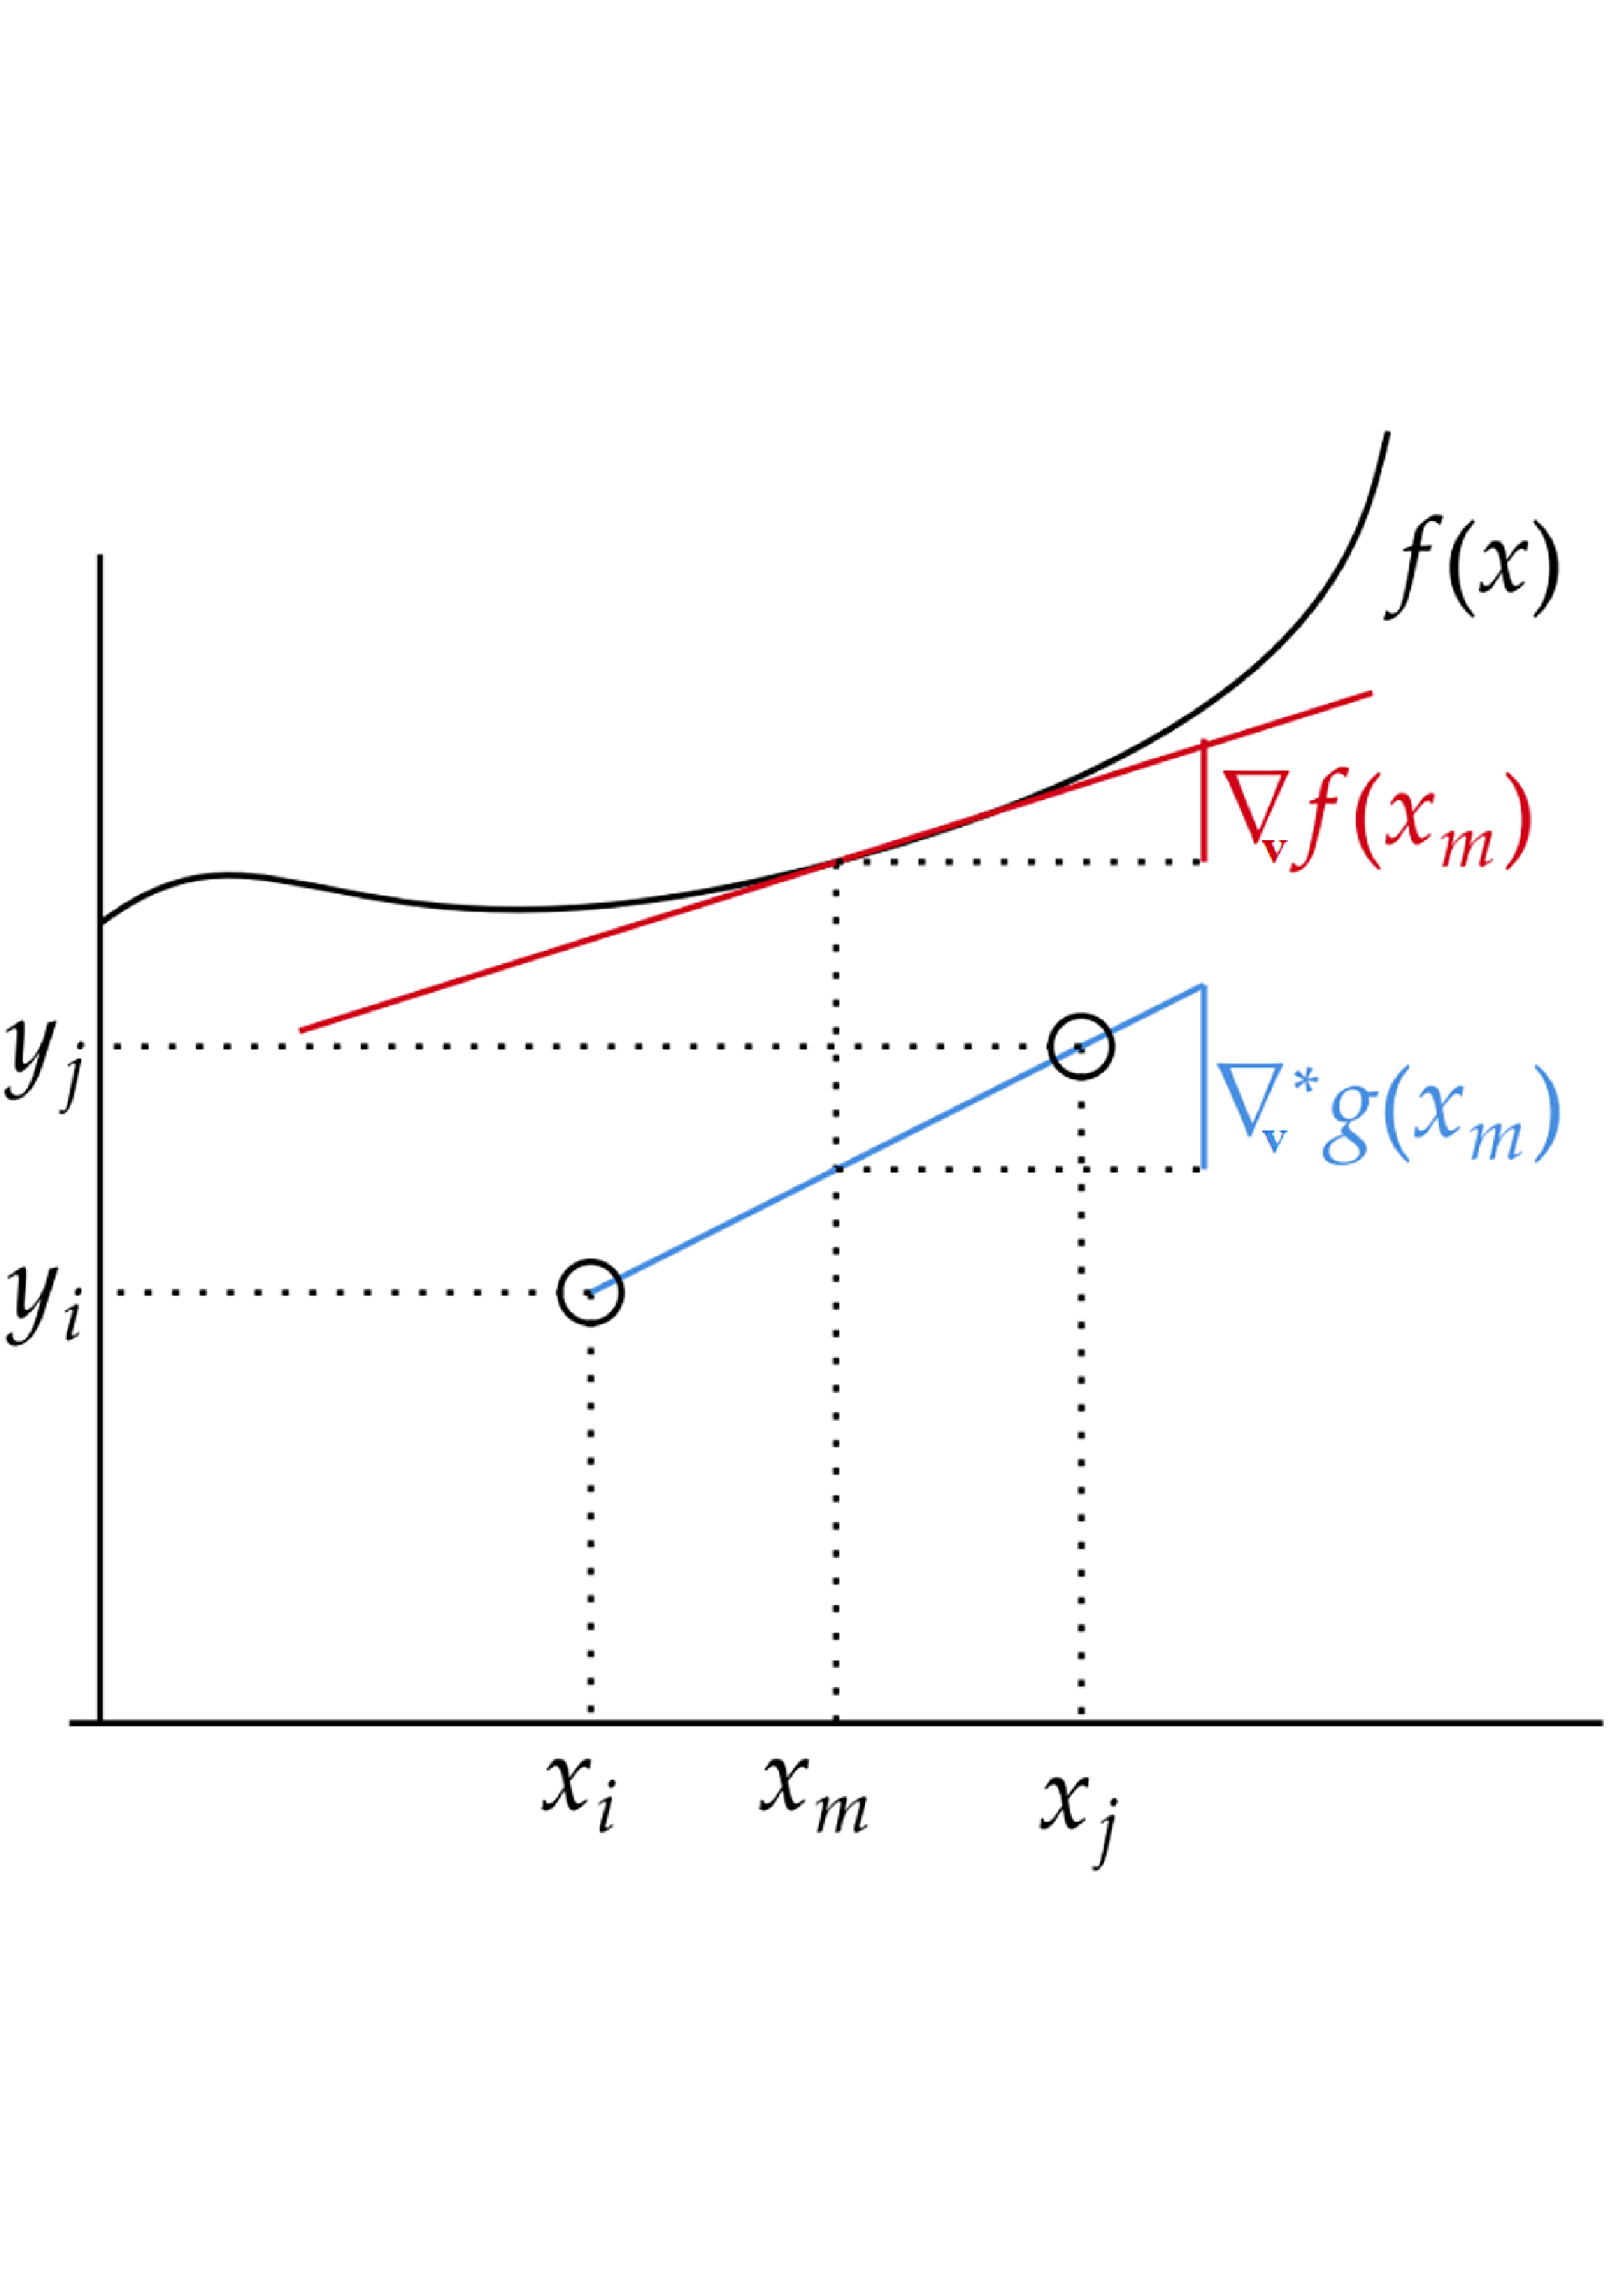
\includegraphics[trim={0cm 8.2cm 0cm 10.3cm},clip,scale=0.2]{diag2.pdf}
 \caption{\emph{DLoss} approach in the one-dimensional case for a tuple of pairs $((\mathbf{x}_i, y_i),(\mathbf{x}_j, y_j))$.
 On the horizontal axis we show the inputs $x$, which are scalars in this example. On the vertical axis, we show the scalar regression targets.
 In general, for a pair of points $\mathbf{x}_i$ and $\mathbf{x}_j$, we calculate the \emph{midpoint} $\mathbf{x}_m = (\mathbf{x}_i+\mathbf{x}_j)/2$ and the difference vector $\mathbf{v} = \mathbf{x}_j - \mathbf{x}_i$.
 The red line shows the model derivative $\nabla_{\mathbf{v}}f(\mathbf{x}_m)$ calculated at $\mathbf{x}_m$.
 The blue line shows the estimated derivative $\nabla^*_{\mathbf{v}}g(\mathbf{x}_m)$ calculated at $\mathbf{x}_m$.
 With \emph{DLoss}, we aim to make the blue and the red lines parallel.
 }
 \label{fig:nablafunct}
\end{figure}

%%%%%%%%%%%%%%%%%%%%%%%%%%%%%%%%%%%%%%%%%%%%%%%%%

\subsection{Derivative Error}\label{subsec_regulmethod}

We propose a new regularization term, the \emph{DLoss}, that is defined on the difference between (an estimate of) the model's derivative and the target's derivative (estimated from the training data).
We use the finite-difference method (FDM) to estimate both derivatives \cite{paszynski2021deep,samaniego2020energy}. 
Intuitively, the main idea of \emph{DLoss} is to align the slope of our model $f(\mathbf{x},\boldsymbol{\beta})$ and the slope of the unknown target function $g(\mathbf{x})$, as illustrated in \autoref{fig:nablafunct}.
Since we are dealing with %continuously differentiable 
functions of multi-dimensional data, we use \emph{directional derivatives}.

\subsubsection{Data Derivative}

In order to calculate the derivative error, we need to estimate the derivative of the unknown target function from the training data. 
For the one-dimensional case, derivatives can be estimated based on neighboring points \cite{kis2021numerical}.
We expand this approach to multi-dimensional feature spaces with the \emph{data derivative}~--- an estimate of the directional derivative of $g$ in the direction of vector $\mathbf{v}$, denoted $\nabla^{*}_{\mathbf{v}}g$. 
When calculating $\nabla^{*}_{\mathbf{v}}g$ we select a tuple, $((\mathbf{x}_i,y_i),(\mathbf{x}_j,y_j))$, from the training data set.
We calculate the \emph{midpoint} $\mathbf{x}_m = (\mathbf{x}_i+\mathbf{x}_j)/2$ between the points $\mathbf{x}_i$ and $\mathbf{x}_j$, and we obtain the difference vector $\mathbf{v} = \mathbf{x}_j - \mathbf{x}_i$.
Then, the data derivative at $\mathbf{x}_m$ along the direction $\mathbf{v}$ is
\begin{equation} 
\nabla^{*}_{\mathbf{v}}g(\mathbf{x}_m) = \frac{y_j - y_i}{\|\mathbf{v}\|_2}\,.
\end{equation}
In general, one cannot give any guarantees as to how far off the estimated derivative $\nabla^{*}_{\mathbf{v}}g$ may be from the true derivative $\nabla_{\mathbf{v}}g$. 
However, $\nabla^{*}_{\mathbf{v}}g(\mathbf{x}_m)$ is the value of the directional derivative at \emph{some} point between $\mathbf{x}_{i}$ and $\mathbf{x}_{j}$. More formally, consider all points $\mathbf{x}_{\tau}$ of the form 
\begin{equation}
 \mathbf{x}_{\tau} = \tau \mathbf{x}_{i} + (1-\tau)\mathbf{x}_{j}
\end{equation} 
with $0\leq\tau\leq1$.
By the mean value theorem e.g., \cite{rodhe-et-al-2012-introduction}, if $g$ is continuous over $\{\mathbf{x}_{\tau}|0\leq\tau\leq1\}$ and differentiable over $\{\mathbf{x}_{\tau}|0<\tau<1\}$, there exists some $\tau$ such that 
\begin{equation}
 \nabla_{\mathbf{v}}g(\mathbf{x}_{\tau}) = \nabla^{*}_{\mathbf{v}}g(\mathbf{x}_m)\,.
\end{equation}



\subsubsection{Model Derivative}

Consider the function $f(\mathbf{x},\boldsymbol{\beta})$, viewed as a function of only $\mathbf{x}$ with fixed $\boldsymbol{\beta}$, and denote this $f(\mathbf{x})$. 
We can obtain the value of $\nabla_{\mathbf{v}}f(\mathbf{x})$---i.e., the directional derivative of $f$ at point $\mathbf{x}$ in the direction of $\mathbf{v}$---either analytically or numerically. 
As with target derivatives, we use an FDM approach to approximate $\nabla_{\mathbf{v}}f(\mathbf{x})$ with $\nabla^{\diamondsuit}_{\mathbf{v}}f(\mathbf{x})$, by calculating%: \kizito{it is incorrect to use a colon after "calculating"} 
\begin{equation} \nabla^{\diamondsuit}_{\mathbf{v}}f(\mathbf{x}) = \frac{ f(\mathbf{x}+\varepsilon\tilde{\mathbf{v}})-f(\mathbf{x}-\varepsilon\tilde{\mathbf{v}})}{2\varepsilon}
\end{equation} 
where $\tilde{\mathbf{v}} = \frac{\mathbf{v}}{\|\mathbf{v}\|_2}$ is normalized to unit length and $\varepsilon$ is a small constant scalar. %\kizito{why aren't we using standard notation for unit vectors, $\hat{\mathbf{v}}$? I had changed it but it has been changed back to $\tilde{\mathbf{v}}$.}\enrico{hi K, we havent touched the hat, however we used tilde because hat is used for y prediction}\kizito{seen and commented out}
This approach is more universal, in the sense that one does not need to determine the directional derivative analytically and (using automatic differentiation) it is easy to implement as a loss function. 

\subsubsection{Tuple Selection}

%For every training pair $(\mathbf{x}_i, y_i)$, $l$ other pairs $(\mathbf{x}_j, y_j)$ with $j \neq i$ are selected to form tuples that are used to calculate $l$ data gradients.
We used two alternative algorithms for selecting tuples. 
Each algorithm, for each training pair $(\mathbf{x}_i, y_i)$, selects $l$ other pairs and, using these pairs, constructs $l$ tuples of the form $((\mathbf{x}_i, y_i), (*, *))$. 
These tuples are used to estimate derivatives in section \ref{subsec_optimization}. %\kizito{I think I understand. Please correct my suggested rephrasing if needed.}\enrico{reads ok}\kizito{seen and commented out}
%\kizito{please rewrite -- this is unclear. The figure uses $l$ to index tuples, but here $l$ indicates a number of pairs.}\tillman{changed letter in text above}\kizito{seen and commented out} 
In \autoref{fig:tuples} we sketch an example of multiple tuples in a multi-dimensional space. 
For training, $l$ is a hyper-parameter. 


\begin{figure}[t]
 \centering
 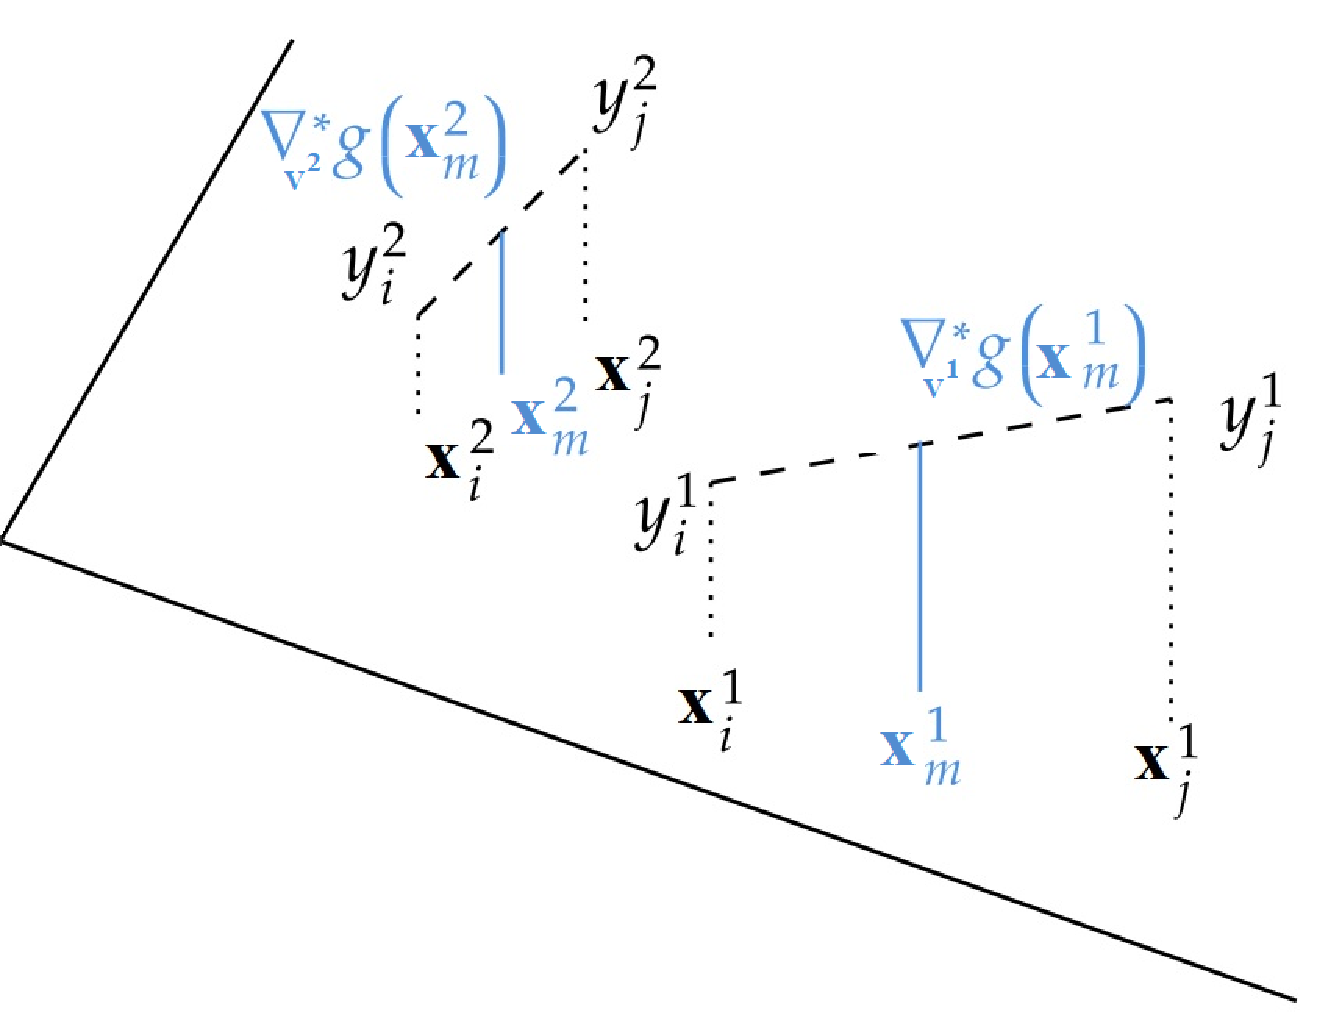
\includegraphics[trim={0cm 0cm 0cm 0cm},clip,scale=0.3]{diag1.pdf}
 \caption{Illustration of data derivatives calculated from two tuples of pairs. 
 For each tuple $((\mathbf{x}^s_i, y^s_i),(\mathbf{x}^s_j, y^s_j))$, where $s\in\{1,2\}$, we calculate the midpoint $\mathbf{x}^s_m$, difference vector $\mathbf{v}^s$, and the corresponding data derivative $\nabla^{*}_{\mathbf{v}^s}g(\mathbf{x}^s_m)$ over a 2-dimensional feature space ($\mathbf{x} \in {\mathbb R}^2$).
%\kizito{as with the other figure, use the full notation (with vector) for directional derivatives that is used in the body of the text. For example, in the figure, use $\nabla^{*}_{\mathbf{v}^2}g(\mathbf{x}^2_m)$.}\kizito{Might be useful, but not necessary, to have a 3rd vertical axis.} \enrico{same here will fix the picture with text notation}\enrico{done and commented}
 }
 \label{fig:tuples}
\end{figure}

\textbf{Nearest neighbor selection}  
For each training pair $(\mathbf{x}_i, y_i)$, we select its $l$ nearest neighbors. The pair $(\mathbf{x}_j,y_j)$, where $j\neq i$, is a nearest neighbor if the distance $\|\mathbf{x}_j-\mathbf{x}_i\|_2$ is minimal.
We determine nearest neighbors using the efficient KD-tree algorithm~\cite{bentley1975multidimensional,nnalgo}. Once a pair is selected as a nearest neighbor, the next nearest neighbor is selected from the remaining pairs in the training set, until $l$ neighbors in total have been selected. 

This approach approximates the derivative based only on local information. 
However, if there is noise in the data (see section \ref{subsec_regressiontasks}) that creates a deviation of $\epsilon$ from the true value of $g(\mathbf{x}_j)-g(\mathbf{x}_i)$, this will lead to 
$ \epsilon / \|\mathbf{x}_j-\mathbf{x}_i\|_2 $ deviation of the estimate $\nabla_\textbf{v}^* g(\mathbf{x}_m)$, so that small distances between points can amplify noise. 

\textbf{Random selection}  
For each training pair $(\mathbf{x}_i, y_i)$, we randomly choose $l$ other pairs from the training set. 
The idea here is that, for noisy data, there is less influence on $\nabla_\textbf{v}^* g(\mathbf{x}_m)$ since the distances between points are greater. 
The trade-off is that greater distances between tuples lead to lower accuracy of the estimated derivatives.

The random selection has $\mathcal{O}(nl)$ time complexity while the nearest neighbors point selection with the KD-tree has $\mathcal{O}(nl + n \log(n))$, which may make random selection preferable for very large datasets.

\subsubsection{Optimization}
\label{subsec_optimization}
The \emph{derivative difference} $dd(\mathbf{x})$ is the amount of of the misalignment between estimated model and target derivatives: 
\begin{equation}
 dd(\mathbf{x}) = \nabla^{\diamondsuit}_{\mathbf{v}}f(\mathbf{x}) - \nabla^{*}_{\mathbf{v}}g(\mathbf{x})\,.
\end{equation}

Let $\mathcal S$ be an index set for all tuples generated by one of the tuple selection approaches above. For the tuple with index $s\in\mathcal S$, we calculate the midpoint, $\mathbf{x}_m^{s}$, and the derivatives' estimates, $\nabla^{\diamondsuit}_{\mathbf{v}^s}f(\mathbf{x}_m^{s})$ and $\nabla^{*}_{\mathbf{v}^s}g(\mathbf{x}_m^{s})$. 
The \emph{DLoss} aggregates the $dd$ values as the mean squared derivative-difference:
\begin{equation}
 DLoss = \frac{1}{|\mathcal S|} \sum_{s\in\mathcal S} dd(\mathbf{x}_m^{s})^2
\end{equation}

where $|\mathcal S|$ is the cardinality of $\mathcal S$. The total loss $L$ for training the model is
\begin{equation}
 L = \theta_{D} DLoss + MSE
\end{equation}
where $\theta_{D}$ is a weighting coefficient. 
This loss is minimized with gradient descent. 

%%%%%%%%%%%%%%%%%%%%%%%%%%%%%%%%%%%%%

\section{Experiments}\label{sec:experiments}

%%%%%%%%%%%%%%%%%%%%%%%%%%%%%%%%%%%%%

\textbf{Setup} In our experiments, the regression model is a simple feed-forward neural network with a single hidden layer of $L_H$ neurons using ReLU activation.
We use ReLU activation because of its popularity in modern neural networks~\cite{goodfellow2016deep}.
The network calculates the function
$\hat{y} = f(\mathbf{x},\boldsymbol{\beta}) =
\sum^{L_H}_{h=1} w_{o,h} r(\mathbf{w}_{h} \cdot \mathbf{x} + b_{h}) + b_{o}$, where $\mathbf{w}_{h}$ and ${b}_{h}$ are the weight vector and bias value of hidden neuron $h$, respectively, and $\cdot$ denotes the scalar product.
The weight between hidden neuron $h$ and the output neuron is $w_{o,h}$ and $b_{o}$ is the bias of the output neuron. 
All of these weights and biases make up the vector $\boldsymbol{\beta}$. 
The rectified linear function (ReLU) $r:\mathbb{R}\rightarrow\mathbb{R}$, defined as $r(x) = max(x,0)$, was to our knowledge first introduced for neural networks  by \cite{fukushima1975relu}. 

In our experiments, we use the Adam optimizer \cite{kingma2015adam}.
We compare the effects of using ${DLoss}$ to $L_2$ and Dropout ($DO$) and no regularization ($STD$). 
We also compare the different variants of tuple selection - Random ($DL_{RND}$) and Nearest neighbors ($DL_{NN}$). 

\textbf{Model parameters} Our models have an input layer with a number of neurons determined by the dimensionality of the datasets, a single hidden layer with $L_H = 64$ hidden neurons, and a single linear output neuron. 
We set $\varepsilon$ to $0.001$ for calculating the model derivative. 

%%%%%%%%%%%%%%%%%%%%%%%%%%%%%%%%%%%%%

\textbf{Data}
In order to observe the effect of our approach in different contexts, we conduct experiments using real data and synthetic, noiseless data. 
Five commonly available real datasets have been selected: Wine, Cancer, Modechoice, Anes96, Diabetes; further information is given in \autoref{tab:data-table}.


\begin{table}[tb]
 \begin{tabular}{llrrcc}
 \toprule
 Name & Type & Inputs & Rows & Library \\
 
 \midrule
 anes96 & Real & 5 & 944 & StM \\
 cancer & Real & 1 & 301 & StM  \\
 diabetes & Real & 10 & 442 & Scikit \\
 modechoice & Real & 6 & 840 & StM  \\
 wine & Real & 11 & 1599 & OpenML  \\
 \cline{2-5} 
 f1 & Synth & 10 & 2500 & Scikit \\
regression1 & Synth & 1 & 2500 & Scikit \\
 regression10 & Synth & 10 & 2500 & Scikit\\
 sparse uncorr & Synth & 10 & 2500 & Scikit\\
 swiss roll & Synth & 3 & 2500 & Scikit  \\

 \bottomrule
 \end{tabular}
 \caption{Datasets used in our experiments. All datasets have a single real-valued output. 
 The number of inputs is listed in column \textsc{Inputs} and \textsc{Rows} is the number of input-output pairs in the dataset. 
 \textsc{Library} describes the Python package from which the dataset is obtained.
 The synthetic datasets (\textsc{Type: Synth}) were generated with the Python library \emph{Scikit-Learn}, version 1.4.1, using the methods from the package $sklearn.datasets$. 
 In the generation of all datasets, no noise has been added.
 Further details of the data generating functions can be found in the library documentation available at \texttt{\textup{https://scikit-learn.org/stable/datasets/}}.
 }
 \label{tab:data-table} 
\end{table}

For noiseless data, we created synthetic datasets starting using data generating functions available from the Scikit-Learn library, where we have selected F1, Regression1, Regression10, Sparse-uncorrelated, Swiss Roll. 
For these, the training data range of the input $\mathbf{x}$ is in the range $[0,1]$ with a fixed $2500$ uniformly distributed points and $1$, $3$, or $10$ features.
\autoref{tab:data-table} shows the main features of the datasets.
We use 5-fold cross validation. 



%%%%%%%%%%%%%%%%%%%%%%%%%%%%%%%%%%%%%

\textbf{Hyper-parameters}
We ran a grid search over the following hyper-parameters: learning rate $\lambda = 0.03,0.01,0.003,0.001$, $L_2$ weight $\theta = 10^{[-3,-4,-5,-6,-7]}$, \emph{DLoss} weight $\theta_{D} = 10^{[-3,-4,-5,-6,-7]}$, and Dropout probability $p = [0.05,0.1,0.2,0.4,0.8]$.
Regularizations $L_2$, $DO$, and \emph{DLoss}, are not combined in our experiments. 
We train our models for 250 epochs and use full batch learning. 

\textbf{Metrics} We report the first epoch at which the best accuracy result is achieved ($ep$) and the time ($t$) for the full training (250 epochs).
The metrics reported are calculated over the 5 cross-validation folds with mean and standard deviation: 
\begin{itemize}
 \item \textbf{$MSE_{train}$}: the average of the best MSE value per fold on the training set over all epochs;
 \item \textbf{$\sigma_{{MSE}_{train}}$}: standard deviation of the best MSE value per fold on the training set over all epochs;
 \item \textbf{$MSE_{val}$}: average of the best MSE value per fold on the validation set over all epochs;
 \item \textbf{$\sigma_{{MSE}_{val}}$}: standard deviation of the best MSE value per fold on the validation set over all epochs;
 \item \textbf{$ep$}: average of the epoch at which the minimum $MSE_{val}$ is reached per epoch;
 \item \textbf{$t$}: average time in seconds to complete a single training per single fold.
\end{itemize}
All experiments were run on a PC with Intel I5 processor and 16GB of RAM running Ubuntu Linux. 

%%%%%%%%%%%%%%%%%%%%%%%%%%%%%%%%%%%%%%%%%%%%%%%

\section{Results}\label{sec:results}

In \autoref{tabresults}, we show the results of our $DL_{RND}$ and $DL_{NN}$ methods as well as $STD$, $L_2$ and $DO$ training. 
$DL_{NN}$ achieves the best generalisation errors $MSE_{val}$ for 5 of the 10 datasets.
The computation time for \emph{DLoss} is generally higher than the $STD$ models (see $t$ values in \autoref{tabresults}).
\autoref{tabranktest} shows the Mean Reciprocal Ranks (MRR) of the different methods with respect to their validation MSE on the datasets. 

\begin{table}[h]
 \begin{center}
 \begin{small}
 \begin{sc}
 \begin{tabular}{llcccc}
 
 \toprule

Dataset & $STD$ & $L_2$& $DO$& $DL_{RND}$& $DL_{NN}$\\

 \midrule
 anes96 & 5 & 3& 4& 2& 1\\
 cancer & 5 & 1& 4& 3& 2\\
 diabetes & 5 & 3& 4& 2& 1\\
 modechoice & 5 & 3& 2& 4& 1\\
 wine & 5& 2& 4& 1& 3\\
 f1 & 5& 1& 3& 4& 2\\
 regression1 & 4& 2& 5& 3& 1 \\
 regression10& 5& 1& 2& 4& 3 \\
 sparse uncorr & 4& 5& 1& 3& 2 \\
 swiss roll & 4& 2& 5& 3& 1 \\
 \hline
 $Avg$& 4.7 & 2.3& 3.4& 2.9& 1.7 \\ 
 \bottomrule
 
 \end{tabular}
 \end{sc}
 \end{small}
 \end{center}
 \caption{The ranks of methods $STD$, $L_2$, $DO$, $DL_{RND}$ and $DL_{NN}$ according to $MSE_{val}$ by $Dataset$ and their averages.}
 \label{tabrank} 
\end{table}

We observe that $DL_{NN}$ has the best MRR, but the difference to $L_2$ is not significant. 
This is not unexpected, considering the small number of datasets. 
However, $DL_{NN}$ errors are significantly lower than $DL_{RND}$, $DO$ and $STD$, and all regularized models are significantly better than $STD$.

\begin{table}[h]
    \begin{center}
    \begin{small}
    \begin{sc}
    
    \begin{tabular}{lr|rrrr}
    \toprule
    Method & MRR & \multicolumn{4}{c}{Significance of differences} \\ 
     &  & \multicolumn{1}{c}{$L_2$} & \multicolumn{1}{c}{$DL_{RND}$} & \multicolumn{1}{c}{$DO$} & \multicolumn{1}{c}{$STD$} \\ \midrule
    $DL_{NN}$ & 0.716 & -  & *  & *  & **  \\
    $L_2$ & 0.570 & & - & - & **  \\
    $DL_{RND}$ & 0.408 & & & - & ** \\
    $DO$ & 0.373 & & & & *  \\
    $STD$ & 0.215 & & & & \\ \bottomrule 
    
    \end{tabular}
    \end{sc}
    \end{small}
    \end{center} 
    \caption{The Mean Reciprocal Rank (MRR, higher is better) values of the different models and their mutual comparisons. `*' or `**' indicate a significant difference, according to a Wilcoxon signed rank test over the results per dataset as shown in \autoref{tabrank}, at the 5\% or 1\% level, respectively.}
    \label{tabranktest}
    
\end{table}


%%%%%%%%%%%%%%%%%%%%%%%%%%%%%%%%%%%%%

\subsection{Discussion}\label{sec:discussion}

In our experiments the $DL_{NN}$ method showed the best results as measured by average rank. 
While the rank difference between $DL_{NN}$ and $L_2$ is not significant, $DL_{NN}$ is significantly better than the $DL_{RND}$ and $DO$, while $L_2$ is not, thus indicating a statistical advantage for $DL_{NN}$ (\autoref{tabranktest}).  
We also analyzed the performance differences in terms of the differences of the validation MSE values, where the differences between $DO$ and $DL_{NN}$ not significant (see \autoref{tabtests}), but we see this as less reliable because the error sizes were quite variable between datasets. 
Overall, there seems to be an advantage to using $DL_{NN}$ that may be worth the additional computation, depending on the application.

It is worth mentioning that the weight $\theta_{D}$ associated with the \emph{DLoss} is on average higher for synthetic data than for real dataset.
We assume that both of these observations relate to the fact that the synthetic datasets are noise-free and the \emph{DLoss} therefore more effective.  

The current finite-difference calculation of the model derivative requires two additional forward-passes per tuple when calculating the derivative, one for $f(\mathbf{x}+\varepsilon\tilde{\mathbf{v}})$ and one for $f(\mathbf{x}-\varepsilon\tilde{\mathbf{v}})$. 
The results in computation times show that all regularization methods require additional computation time on average, but that the amount is quite variable.
It may be possible to reduce the cost by not determining the model derivative at the midpoint but reusing data points instead or by using analytical gradient calculations, which would be model dependent. 

Overall, both the performance and the computation time warrants further experimentation, including different machines, different models and combinations of different regularization methods. 


\begin{table}[h]
 \begin{center}
 \begin{small}
 \begin{sc}
 \begin{tabular}{c|llll}
 
 \toprule
 Group & $Median_{\Delta}$ & Wilcoxon $p$ \\
 
 \midrule
 Real $STD$ $DL_{RND}$ & 1.3$\times10^{-2}$ & $0.035^{*}$  \\
 Real $STD$ $DL_{NN}$ & 4.2$\times10^{-2}$ & 0.078 \\
 Real $L_2$ $DL_{RND}$ & -8.6$\times10^{-3}$ & 0.53  \\
 Real $L_2$ $DL_{NN}$ & -4.1$\times10^{-4}$ & 0.32  \\
 Real $DO$ $DL_{RND}$ & 1.8$\times10^{-2}$ & 0.19 \\
 Real $DO$ $DL_{NN}$ & 4.5$\times10^{-3}$ & 0.25 \\
 
 \hline
 Synthetic $STD$ $DL_{RND}$ & 3.9$\times10^{-5}$ & $0.005^{**}$ \\
 Synthetic $STD$ $DL_{NN}$ & 1.8$\times10^{-5}$ & $0.011^{*}$  \\
 Synthetic $L_2$ $DL_{RND}$ & -2.9$\times10^{-5}$ & 0.85 \\
 Synthetic $L_2$ $DL_{NN}$ & -2.7$\times10^{-5}$ & 0.77 \\
 Synthetic $DO$ $DL_{RND}$ & 6.9$\times10^{-6}$ & 0.42  \\
 Synthetic $DO$ $DL_{NN}$ & 1.2$\times10^{-5}$ & 0.26  \\
 
 \bottomrule

 
 \toprule
 Group &  Shapiro-Wilk $p$ & t-test $p$\\
 
 \midrule
 Real $STD$ $DL_{RND}$ & $0.046^{*}$ & $0.057$ \\
 Real $STD$ $DL_{NN}$ & 0.37 & $0.044^{*}$\\
 Real $L_2$ $DL_{RND}$ & 0.75 & 0.48 \\
 Real $L_2$ $DL_{NN}$ & $0.022^{*}$ & 0.28 \\
 Real $DO$ $DL_{RND}$ & $0.017^{*}$ & 0.38 \\
 Real $DO$ $DL_{NN}$ & 0.56 & 0.21 \\
 
 \hline
 Synthetic $STD$ $DL_{RND}$ & 3.6$\times10^{-6***}$ & 0.157\\
 Synthetic $STD$ $DL_{NN}$  & 2.3$\times10^{-5***}$ & 0.121 \\
 Synthetic $L_2$ $DL_{RND}$ & 6.7$\times10^{-6***}$ & 0.241\\
 Synthetic $L_2$ $DL_{NN}$ & 5.6$\times10^{-7***}$ & 0.144\\
 Synthetic $DO$ $DL_{RND}$ & 7.3$\times10^{-6***}$ & 0.86 \\
 Synthetic $DO$ $DL_{NN}$ & 2.2$\times10^{-6***}$ & 0.49 \\
 
 \bottomrule
 \end{tabular}
 
 \end{sc}
 \end{small}
 \end{center}

 \caption{The results of significance tests for differences of $MSE_{val}$ between $STD$ and \emph{DLoss} results. 
 We run the tests on the difference of the standard learning method group - $STD$ group - and the group with \emph{DLoss} - $DL$ group.
 For both $STD$ and $DL$ training we have 2 group, therefore we run all combinations, giving us 6 results, for real data and synthetic.
 We compare each of the 5-fold in the cross validation for each of the 5 datasets, thus 25 samples per test.
 $Median_{\Delta}$ is the median of pairwise difference between the $MSE_{val}$ values of the groups.
 We applied the Wilcoxon Signed Ranked Test, a non-parametric test for significance of differences between the medians. 
 The low $p$-values of the signed rank test indicate that the $STD$ groups' $MSE_{val}$ is significantly greater than the and $DL$ groups' (indicated with an asterisk *). 
 The $^{*},^{**},^{***}$ indicate the significance at 5\%, 1\% and 0.1\% 
 confidence, respectively.
 We also applied a paired t-test. 
 However, the t-test is only strictly valid for normally distributed data, and the Shapiro-Wilk test indicates that the distribution is significantly different from a normal distributions. 
 }
 \label{tabtests}
\end{table}

%%%%%%%%%%%%%%%%%%%%%%%%%%%%%%%%%%%%%

\section{Conclusion}\label{sec:conclusion}
We propose a new regularization method, \emph{DLoss}, which aims to reduce the difference between model derivatives and target function derivatives by using differential information inferred from training data.
The \emph{DLoss} method is tested on ten regression datasets.
We propose two versions of the method with different tuple-selection algorithms~--- random and nearest neighbor selection.
We experiment on a neural network with a single hidden layer, multiple inputs, and a single output. 
We use the MSE error on validation sets to compare the performance of different regularization methods. 
We observe an overall generalization improvement using \emph{DLoss} with nearest neighbor selection ($DL_{NN}$). 
With this method, the generalization as measured by average rank is better than the established $L_2$ and Dropout regularization. 

The improved generalization requires additional computation, but the results in practice are quite variable between the different regularization methods and algorithmic optimizations may help to reduce the cost. 
Future on this approach work will include tests with more models and more datasets and exploration of combined regularization methods as well as the formulation of \emph{DLoss} for classification problems.
Higher dimensional datasets with more data points and more model architectures will be explored in order to determine how far the benefits of using the \emph{DLoss} method generalize. 


%%%%%%%%%%%%%%%%%%%%%%%%%%%%%%%%%%%%%

\bibliographystyle{apalike} 
\bibliography{references} 

\onecolumn

%%%%%%%%%%%%%%%%%%%%%%%%%%



%%%%%%%%%%%%%%%%%%%%%%%%%%

\begin{table}
 \begin{center}
 \begin{small}
 \begin{sc}
 \npdecimalsign{.}
 \nprounddigits{5}
 \begin{tabular}{ll n{1}{5} n{1}{5} n{1}{5} n{1}{5} rr}
 
 \toprule
 Dataset & Method & \multicolumn{1}{c}{$MSE_{{train}}$} & \multicolumn{1}{c}{$\sigma_{{train}}$} & \multicolumn{1}{c}{$MSE_{{val}}$} & \multicolumn{1}{c}{$\sigma_{{val}}$} & $ep$ & $t$ \\
 
 \midrule
\multirow{5}{*}{anes96} & $STD$ & 0.177330 & 0.019518 & 0.60008727 & 0.11239327 & 15 & 2.6 \\
 & $L_2$ & 0.30780832 & 0.02352047 & 0.57475274 & 0.09235593 & 41 & 7.7 \\
 & $DO$ & 0.49298516 & 0.03259643 & 0.58150342 & 0.13898003 & 53 & 2.6\\
 & $DL_{RND}$ & 0.19896433 & 0.01540072 & 0.56350781 & 0.1194641 & 12 & 5.5\\
 & $DL_{NN}$ & 0.4295374 & 0.03931913 & {\npboldmath}0.56324297 & 0.09467875 & 53 & 11.8\\ \cline{2-8}
\multirow{5}{*}{cancer} & $STD$ & 0.29283602 & 0.01398396 & 0.24764358 & 0.24436089 & 17 & 2.2 \\
 & $L_2$ & 0.30778304 & 0.03125095 & {\npboldmath}0.21662021 & 0.21220799 & 98 & 2.2 \\
 & $DO$ & 0.29449674 & 0.01644076 & 0.23368603 & 0.20838813 & 105 & 7.8 \\
 & $DL_{RND}$ & 0.29207851 & 0.02132386 & 0.22473886 & 0.18396828 & 84 & 3.9 \\
 & $DL_{NN}$ & 0.30993664 & 0.03188799 & 0.21857888 & 0.16864872 & 77 & 3.7 \\ \cline{2-8}
\multirow{5}{*}{diabetes} & $STD$ & 0.33635206 & 0.05040892 & 0.50646346 & 0.17958295 & 113 & 2.3 \\
 & $L_2$ & 0.14309196 & 0.04330189 & 0.45751889 & 0.11661063 & 43 & 5.3 \\
 & $DO$ & 0.38423959 & 0.01592457 & 0.47632056 & 0.131764 & 133 & 13.7 \\
 & $DL_{RND}$ & 0.11744604 & 0.02434119 & 0.45636614 & 0.17695314 & 32 & 4.3 \\
 & $DL_{NN}$ & 0.00893422 & 0.00529294 & {\npboldmath}0.4553714 & 0.23124737 & 23 & 5.9 \\ \cline{2-8}
\multirow{5}{*}{modechoice} & $STD$ & 0.1179477 & 0.01804242 & 0.63944455 & 0.14480025 & 131 & 2.6\\
 & $L_2$ & 0.14903403 & 0.03706822 & 0.58849685 & 0.05570832 & 179 & 7.5 \\
 & $DO$ & 0.44150581 & 0.01733288 & 0.53832477 & 0.07132203 & 186 & 15.4 \\
 & $DL_{RND}$ & 0.13025415 & 0.01307876 & 0.59405038 & 0.08625778 & 99 & 9.1 \\
 & $DL_{NN}$ & 0.14156311 & 0.01416364 & {\npboldmath}0.53603314 & 0.16874024 & 147 & 8.8 \\ \cline{2-8}
\multirow{5}{*}{wine} & $STD$ & 0.09746584 & 0.01039641 & 0.59575467 & 0.11823012 & 17 & 3.1 \\
 & $L_2$ & 0.08724606 & 0.00577489 & 0.55471867 & 0.13983683 & 31 & 43.3 \\
 & $DO$ & 0.44190202 & 0.01508975 & 0.5916705 & 0.16977146 & 117 & 93.7 \\
 & $DL_{RND}$ & 0.47699501 & 0.02936241 & {\npboldmath}0.5496235 & 0.23304432 & 167 & 15.1 \\
 & $DL_{NN}$ & 0.11576753 & 0.00938199 & 0.56862197 & 0.13514901 & 36 & 16.3 \\ \cline{2-8}
\multirow{5}{*}{f1} & $STD$ & 0.00143714 & 0.00022515 & 0.00854035 & 0.08697299 & 241 & 3.7 \\
 & $L_2$ & 0.00136922 & 0.00013204 & {\npboldmath}0.0063039 & 0.08154564 & 248 & 45.8 \\
 & $DO$ & 0.01164792 & 0.00038945 & 0.00673393 & 0.08439192 & 242 & 3.5 \\
 & $DL_{RND}$ & 0.00138717 & 0.00032696 & 0.00688173 & 0.05618682 & 245 & 10.2 \\
 & $DL_{NN}$ & 0.00137461 & 0.00014238 & 0.00655821 & 0.00045686 & 250 & 23.2 \\ \cline{2-8}
\multirow{5}{*}{regression1} & $STD$ & 7.14e-6 & 4.03e-6 & 7.64e-6& 0.02236516 & 250 & 3.6\\
 & $L_2$ & 4.93e-6 & 2.3e-6 & 4.84e-6& 0.07453147 & 250 & 44.6\\
 & $DO$ & 0.00274638 & 0.00014872 & 1.459e-5 & 0.0344513 & 217 & 3.5 \\
 & $DL_{RND}$ & 5.26e-6 & 2.93e-6 & 5.86e-6& 0.03172563 & 249 & 10.1\\
 & $DL_{NN}$ & 4.15e-6 & 2.66e-6 & {\npboldmath}4.19e-6& 0.08469988 & 250 & 23.8\\ \cline{2-8}
\multirow{5}{*}{regression10} & $STD$ & 0.00012851 & 3.658e-5 & 0.00042876 & 0.13315077 & 250 & 3.7 \\
 & $L_2$ & 2.228e-5 & 8.8e-7 & {\npboldmath}2.652e-5 & 0.07846928 & 250 & 57.7\\
 & $DO$ & 0.00451834 & 0.00022454 & 0.0001753 & 0.13754859 & 235 & 3.5\\
 & $DL_{RND}$ & 0.000138 & 2.24e-5 & 0.00039169 & 0.08767906 & 249 & 24.4\\
 & $DL_{NN}$ & 0.0001294 & 2.35e-5 & 0.00037651 & 9.917e-5 & 250 & 9.7 \\ \cline{2-8}
\multirow{5}{*}{sparse uncorr} & $STD$ & 0.05514032 & 0.0030176 & 0.08518794 & 0.06130903 & 174 & 3.7 \\
 & $L_2$ & 0.02399948 & 0.00171738 & 0.08620409 & 0.09918734 & 42 & 3.8\\
 & $DO$ & 0.17109021 & 0.00405457 & {\npboldmath}0.07938602 & 0.04937745 & 197 & 3.5\\
 & $DL_{RND}$ & 0.0381035 & 0.0025631 & 0.08294402 & 0.14912423 & 45 & 10.0\\
 & $DL_{NN}$ & 0.02399658 & 0.00205902 & 0.08209252 & 0.07535213 & 44 & 23.8 \\ \cline{2-8}
\multirow{5}{*}{swiss roll} & $STD$ & 0.0001703 & 3.736e-5 & 0.00023135 & 0.10705988 & 249 & 3.7\\
 & $L_2$ & 0.00013068 & 4.676e-5 & 0.00016883 & 0.05157496 & 248 & 39.8\\
 & $DO$ & 0.01236847 & 0.00051966 & 0.00108743 & 0.03987374 & 210 & 3.5\\
 & $DL_{RND}$ & 0.00013275 & 2.252e-5 & 0.00019632 & 0.03456687 & 245 & 23.8\\
 & $DL_{NN}$ & 0.00012357 & 2.436e-5 & {\npboldmath}0.00016706 & 2.355e-5 & 239 & 9.5\\ 
 
 \bottomrule
 \end{tabular}
 \npnoround
 \end{sc}
 \end{small}
 \end{center}

 \caption{$Data$, $Method$ and $Metrics$ of experiments as mean of best results in 5-fold cross validation over 250 epochs. Neural network of multiple inputs and single output. Network structure of 64 hidden neurons and ReLU activation function. Comparison of $STD$, $L_2$, $DO$ vs $DL_{RND}$ random selection and vs $DL_{NN}$ nearest neighbour selection. 
 In bold are highlighted the best results per datasets. 
 }
 \label{tabresults}
\end{table}


%%%%%%%%%%%%%%%%%%%%%%%%%%%%%%%%%%%%%%%%


\end{document}
